\documentclass[12pt]{book} 

\usepackage{amsmath}
\usepackage{graphicx}
\usepackage{import}
\usepackage{amsfonts}
\usepackage{booktabs}

\setlength{\parindent}{0em}  % sets auto indent at new paragraph to none

\newcommand{\incfig}[1]{%
    \import{./figures/}{#1.pdf_tex}
}

\title{\coursetitle\linebreak\lecturename}
\author{\\Cain Susko\\ 
           \\ \\ \\
      Queen's University 
    \\School of Computing\\} 

%=-=-=-=-=-title-=-=-=-=-=%
\newcommand{\lecturename}{Machine Representation of Programs: Procedures 2}
\newcommand{\coursetitle}{Computer Architecture}
%=-=-=-=-=-#####-=-=-=-=-=%

\begin{document}
\begin{titlepage}
        \maketitle
\end{titlepage}


\section*{Recall}
recall the stack frame for x86-64 linux systems:
\begin{figure}[h]
        \centering
        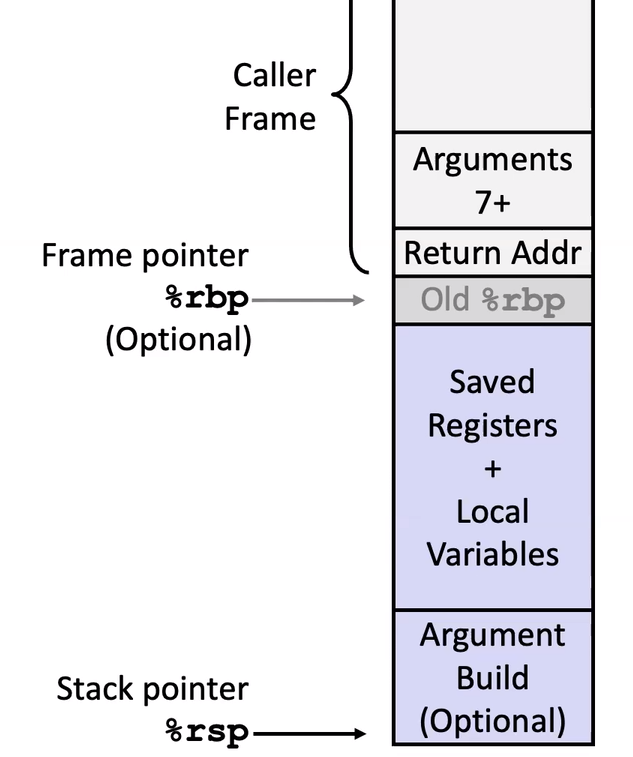
\includegraphics[scale = 0.4]{./figures/linuxstack}
\end{figure}

Additionally, recall the example \texttt{incr}:

\begin{figure}[h]
        \centering
        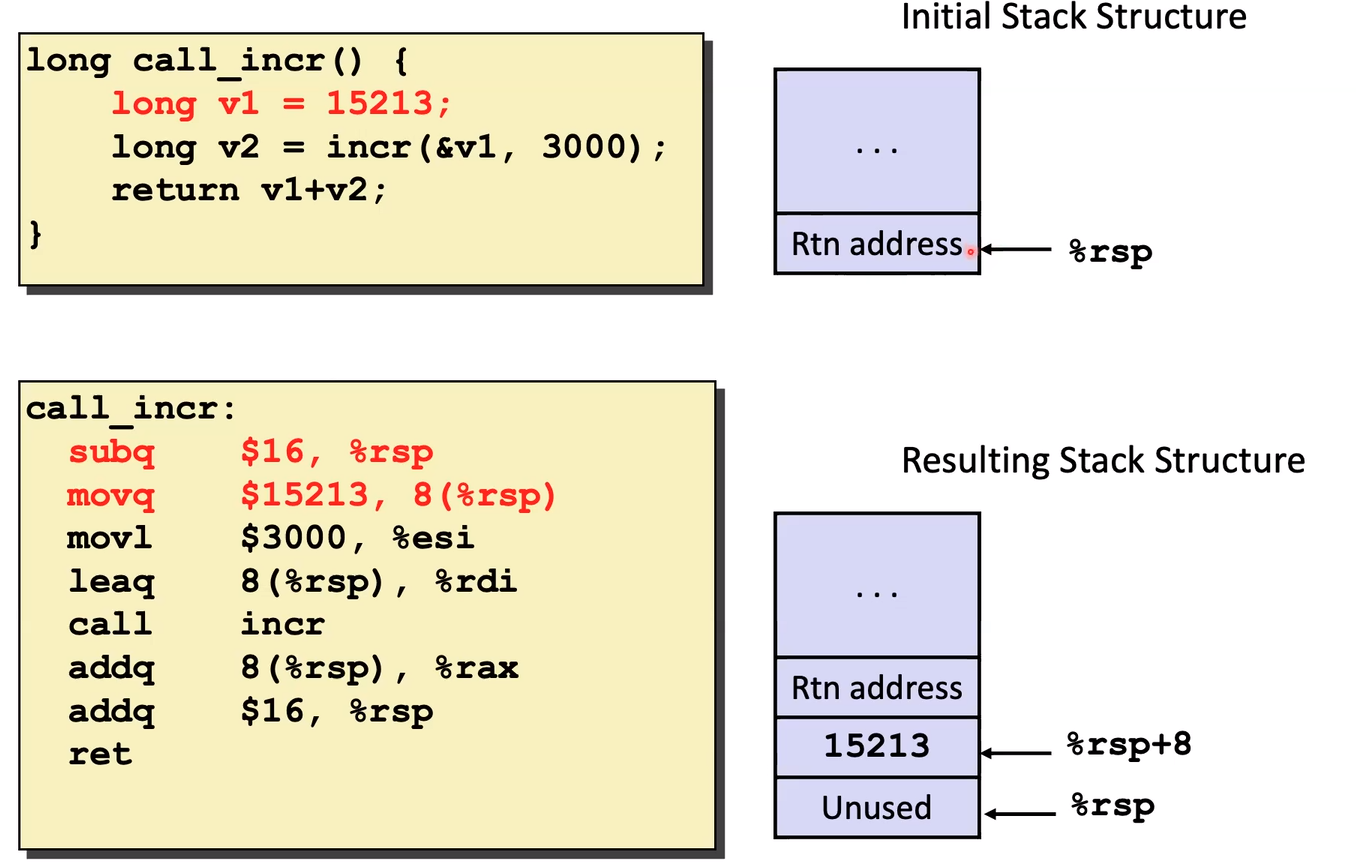
\includegraphics[scale = 0.1]{./figures/incr1}
        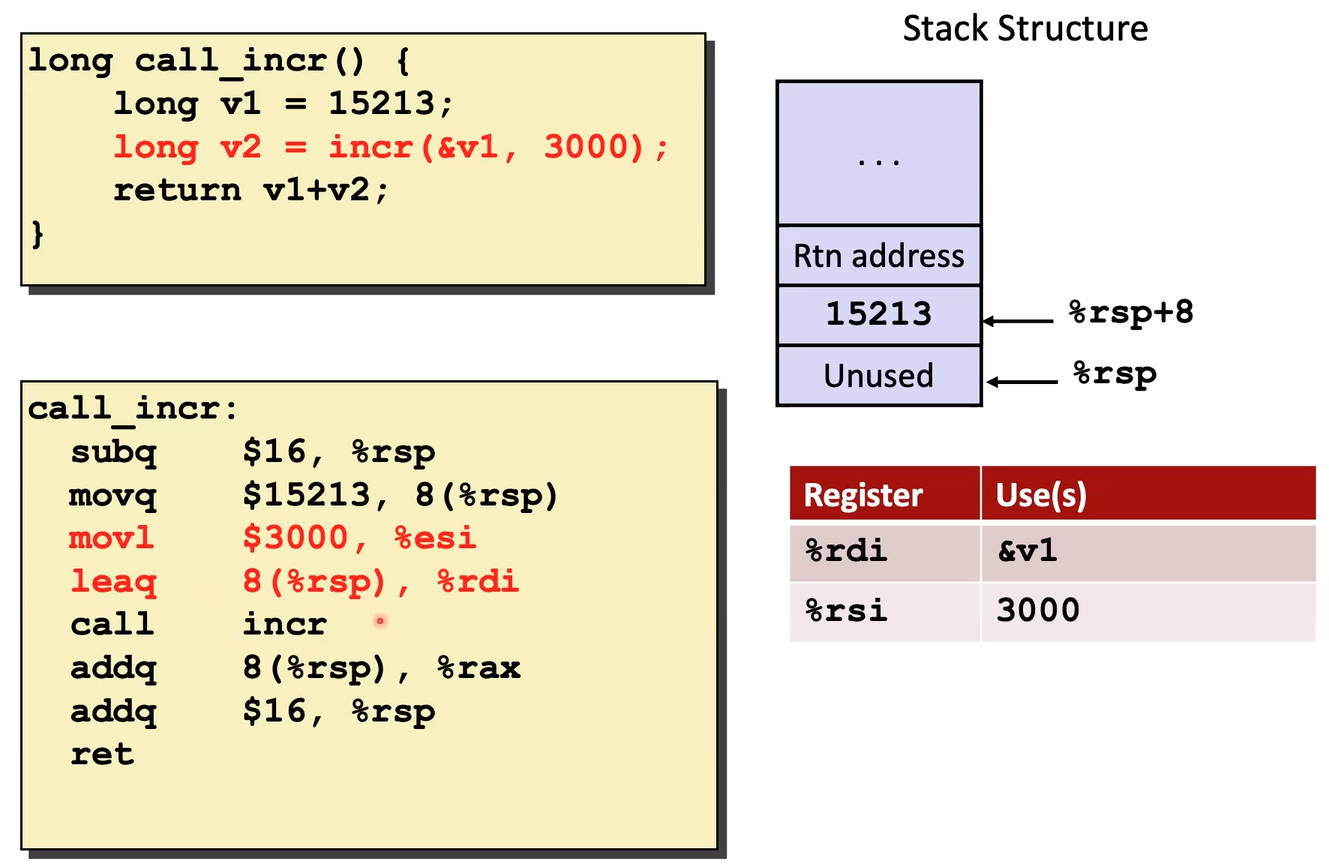
\includegraphics[scale = 0.1]{./figures/incr2}
        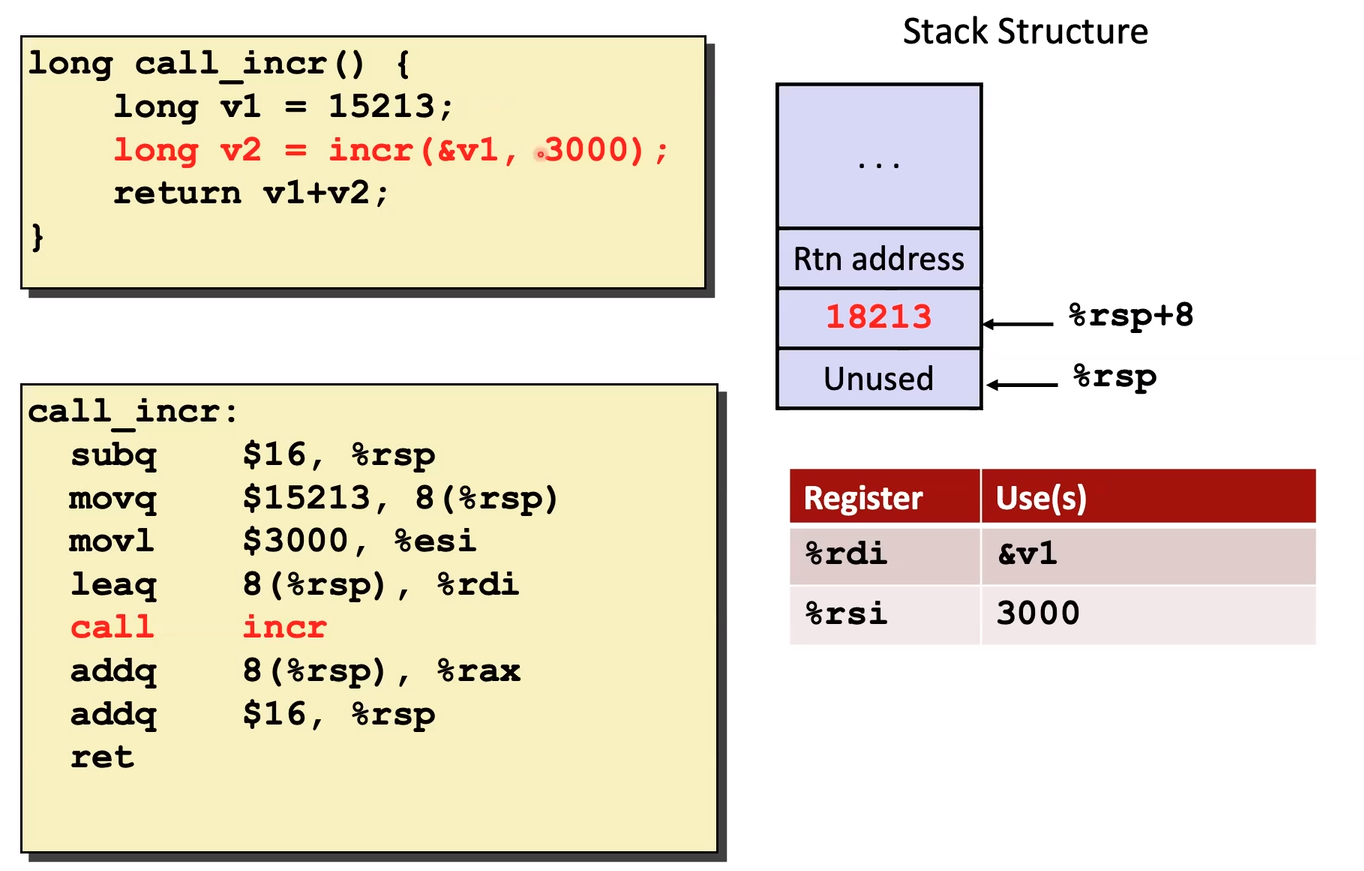
\includegraphics[scale = 0.1]{./figures/incr3}
        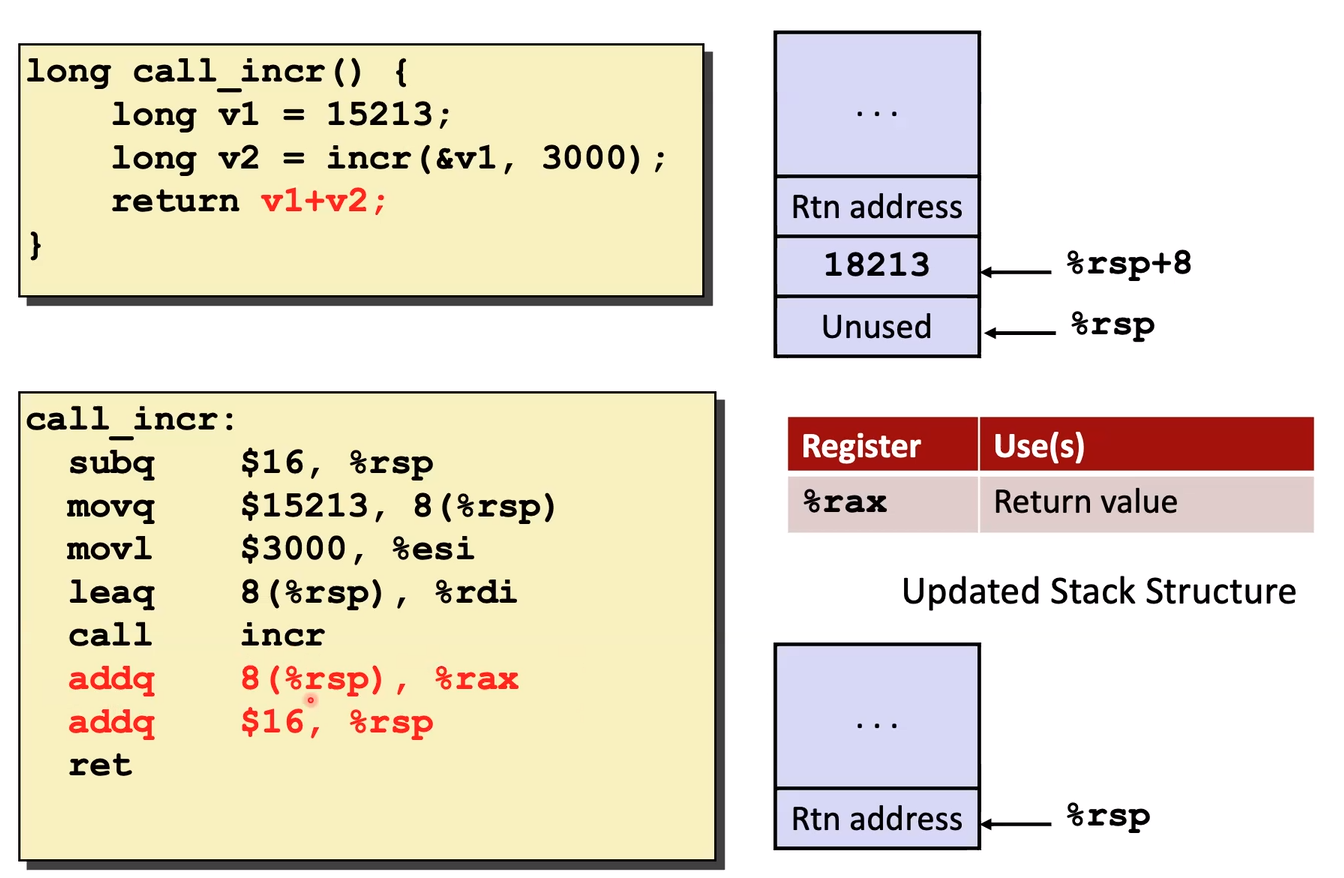
\includegraphics[scale = 0.1]{./figures/incr4}
        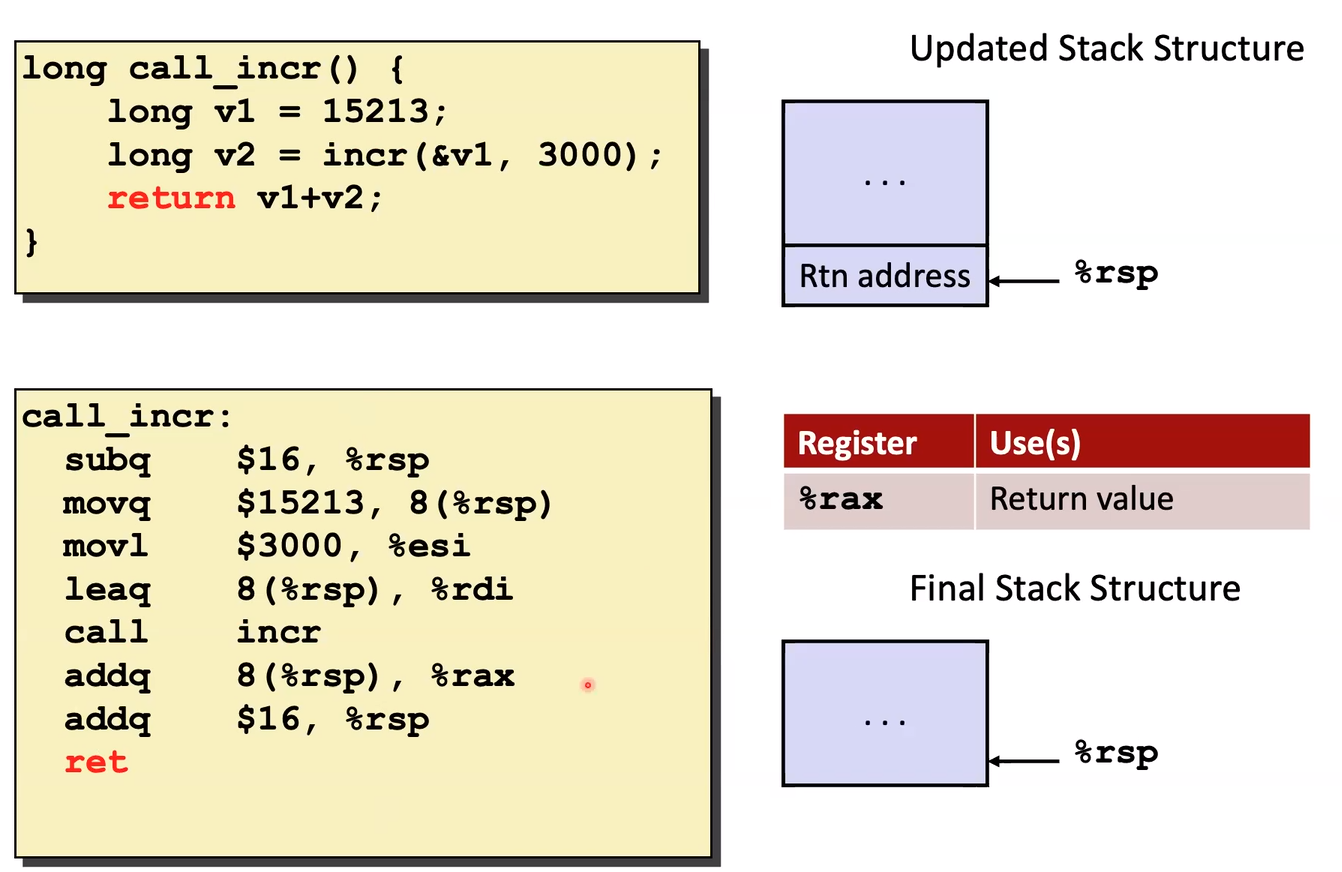
\includegraphics[scale = 0.1]{./figures/incr5}
\end{figure}

\section*{Register Saving Conventions}
There are 2 main conventions when saving registers:
\begin{align*}
        &\text{Caller Saved} &\text{caller saves temp vals in frame before call}\\
        &\text{Callee Saved} &\text{callee saves temp vals in frame before using them}\\
        & &\text{callee then restores vals before returning to caller}
.\end{align*}

These conventions are defined within the architecture its self. 

Within a Linux x86-64 system, the registers
are used like so:
\begin{figure}[h]
        \centering
        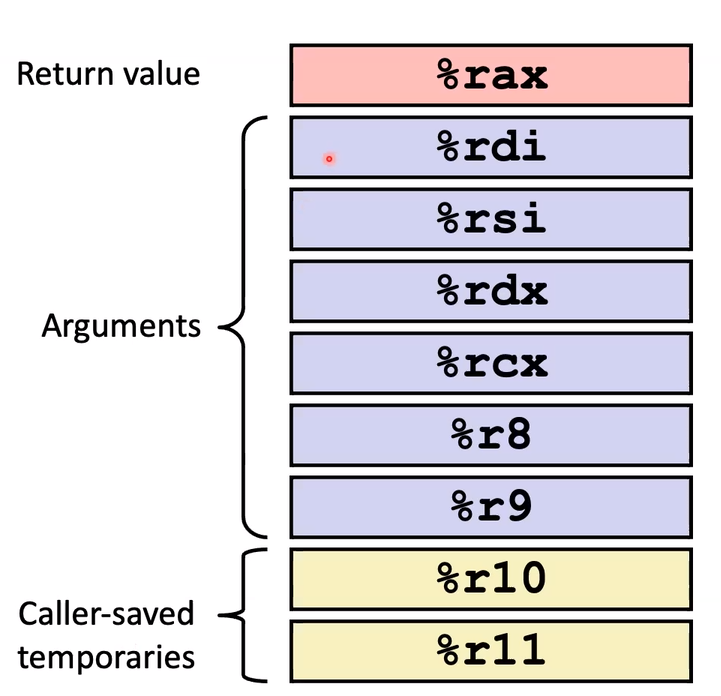
\includegraphics[scale = 0.3]{./figures/linuxreg1}
        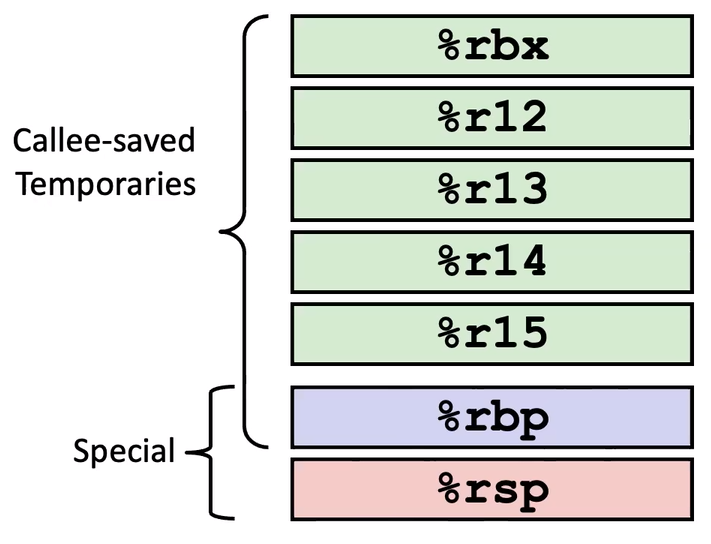
\includegraphics[scale = 0.3]{./figures/linuxreg2}
\end{figure}

Where:
\begin{itemize}
        \item \texttt{\%rax} is caller saved and can be modified by procedure
        \item \texttt{\%rdi,\ldots, \%r9} are also caller saved but can be modified by the callee procedure.
        \item \texttt{\%r10, \%r11} are caller saved and can be modified by callee procedure.
        \item \texttt{\%rbx,\ldots,\%r15} is callee saved. The callee must save and restore the data (push and pop to
                stack)
        \item \texttt{\%rbp} is callee saved and the callee must save and restore the register. Additionally, 
                it can be used as a frame pointer.
        \item \texttt{\%rsp} special form of callee save where it is restored to original value upon exit from procedure
\end{itemize}
\pagebreak

For Example:
\begin{figure}[h]
        \centering
        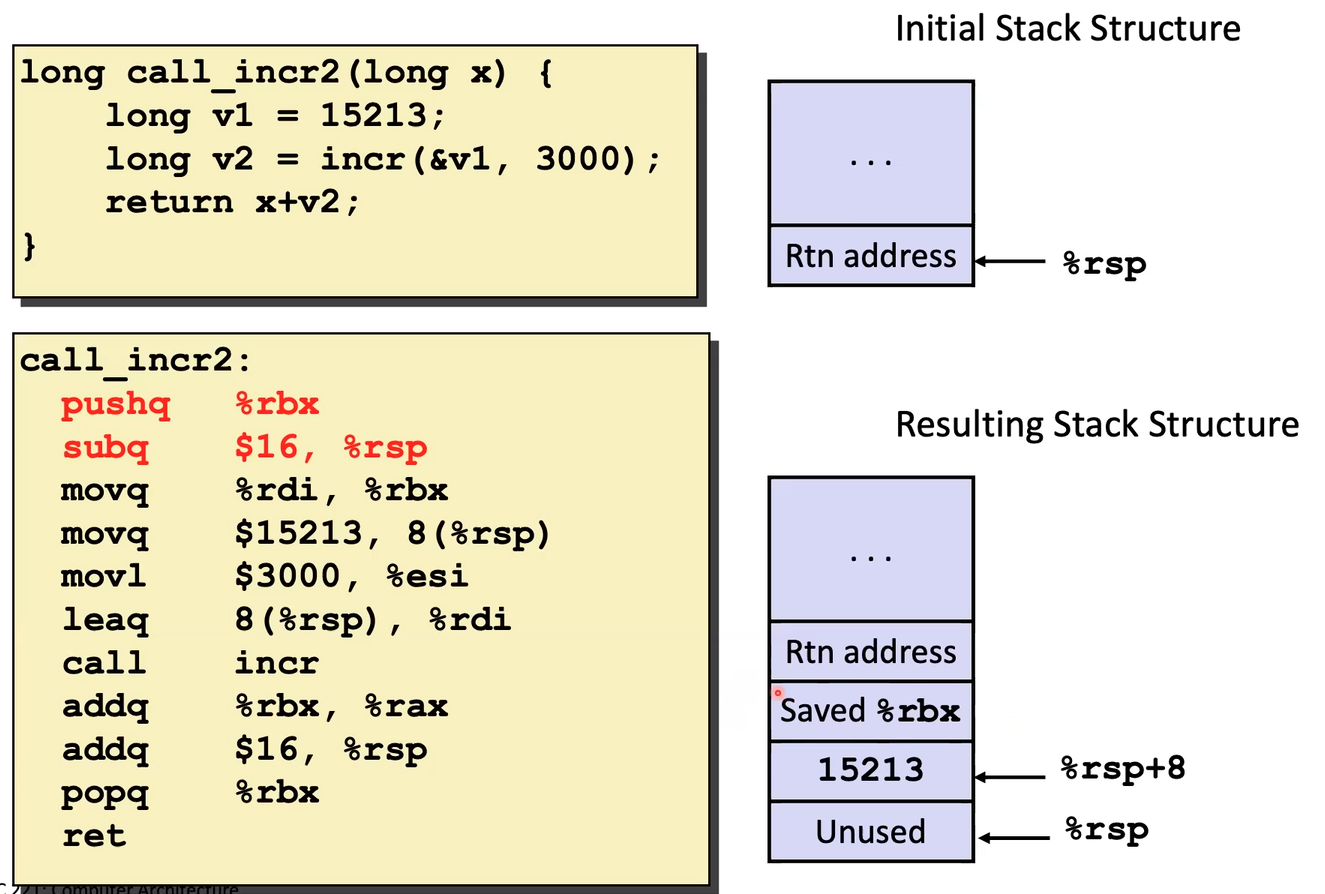
\includegraphics[scale = 0.3]{./figures/saveEx1}
        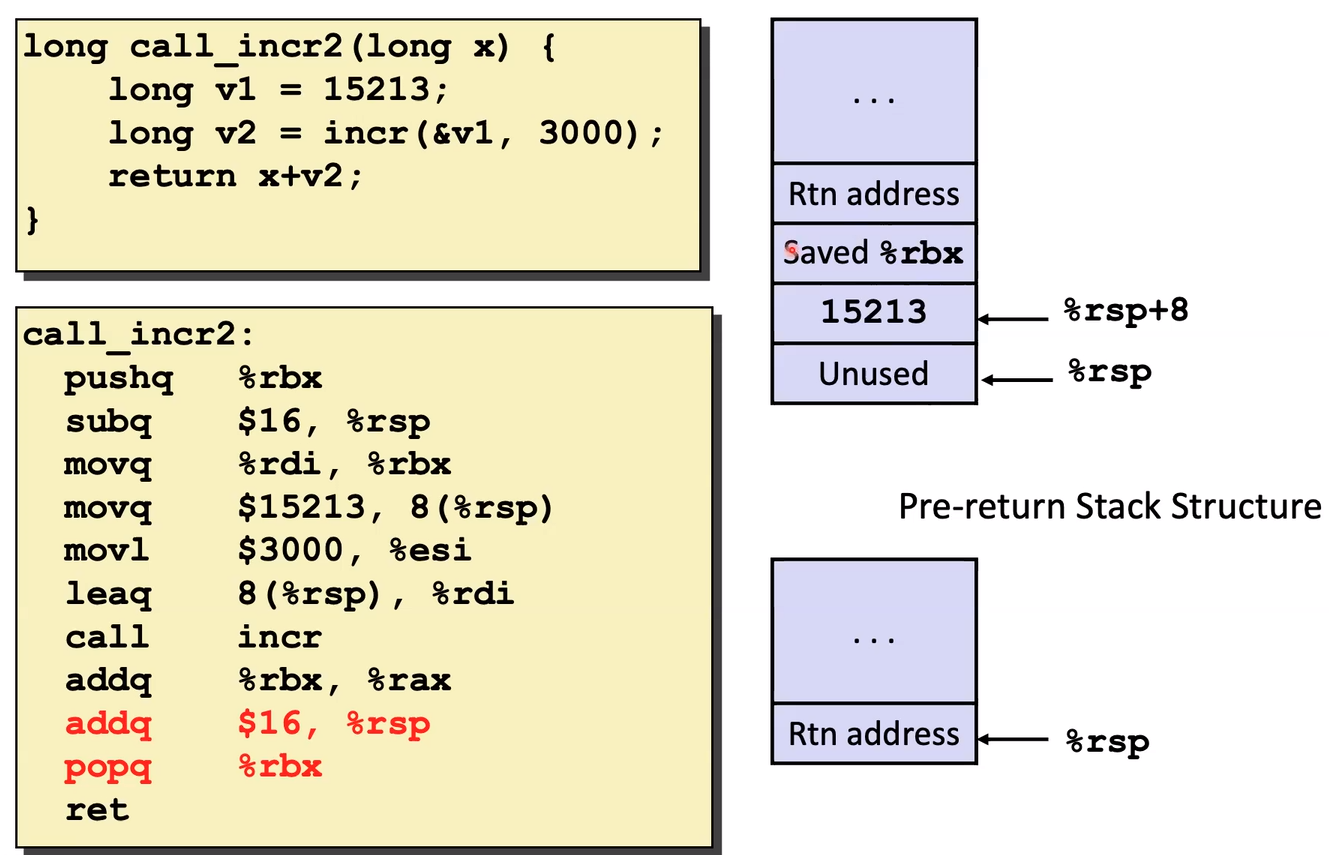
\includegraphics[scale = 0.3]{./figures/saveEx2}
\end{figure}

\pagebreak

\section*{Recursive Functions \& the Stack}
Finally, the behaviour that a recursive function has within this structure of registers, stacks, and frames is
shown by the following example:
\begin{figure}[h]
        \centering
        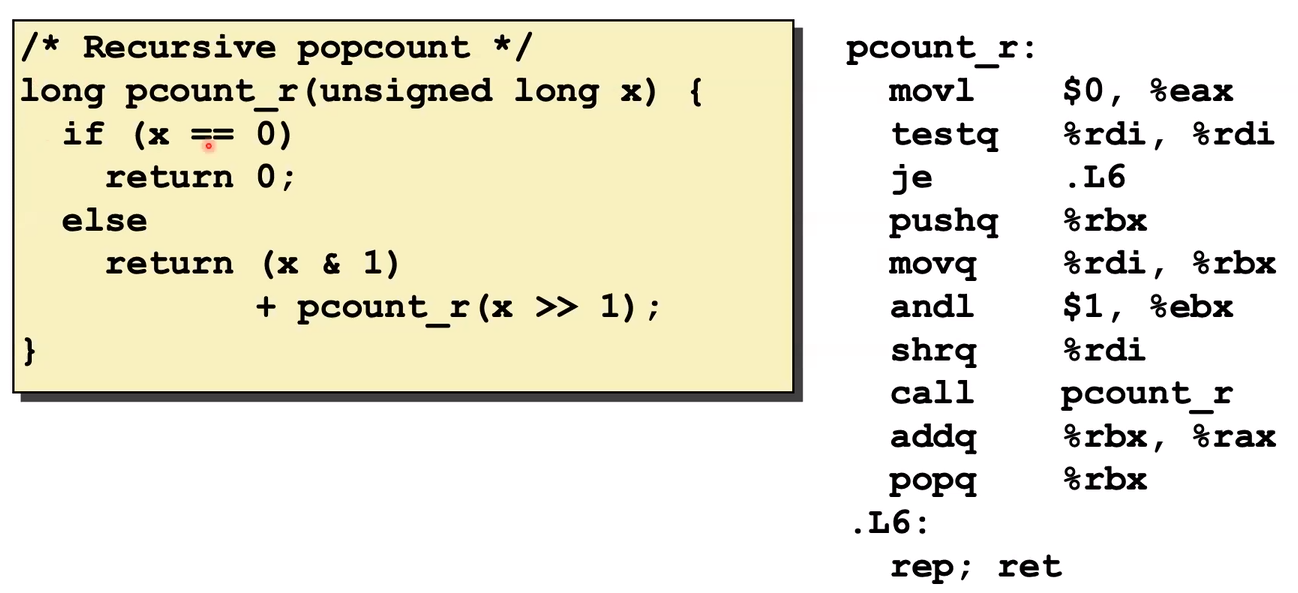
\includegraphics[scale = 0.2]{./figures/rec1}
\end{figure}

\begin{figure}
        \centering
        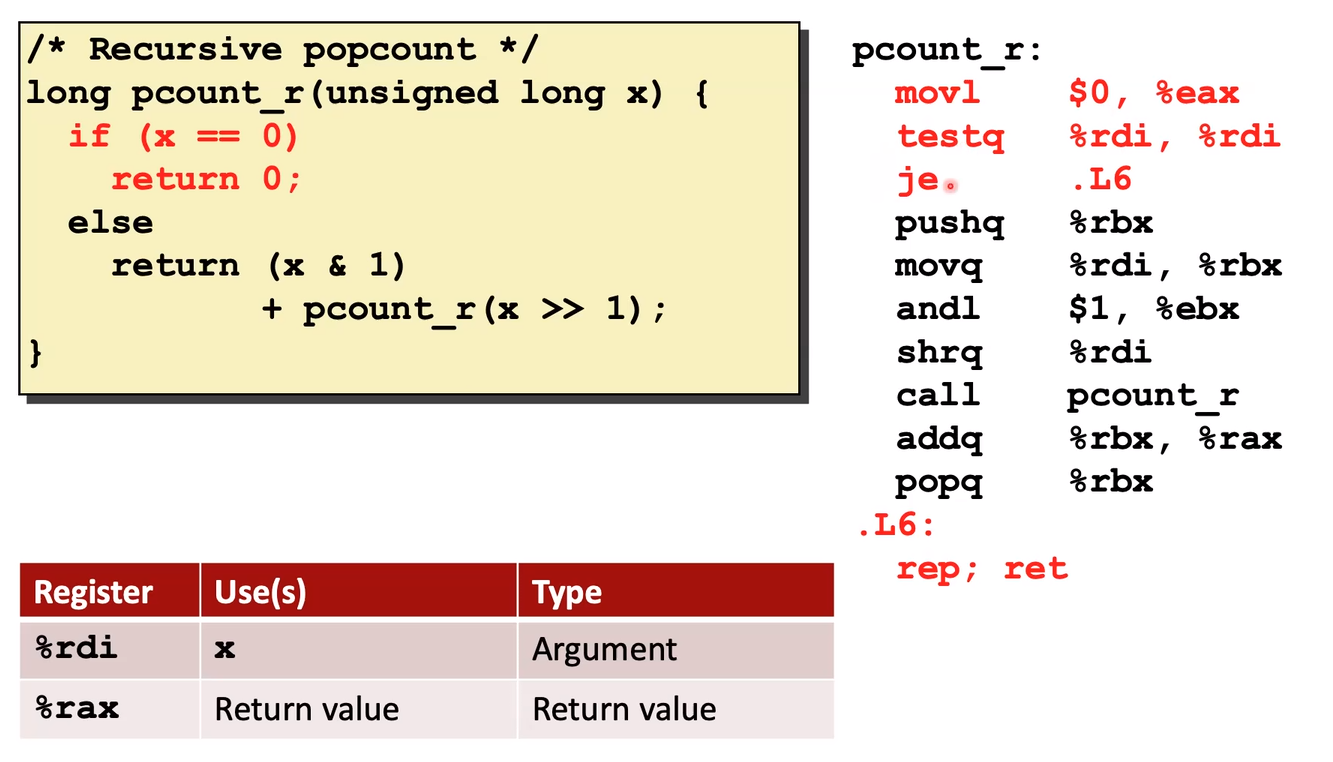
\includegraphics[scale = 0.2]{./figures/rec2}
        \caption{terminal case}
\end{figure}

\begin{figure}
        \centering
        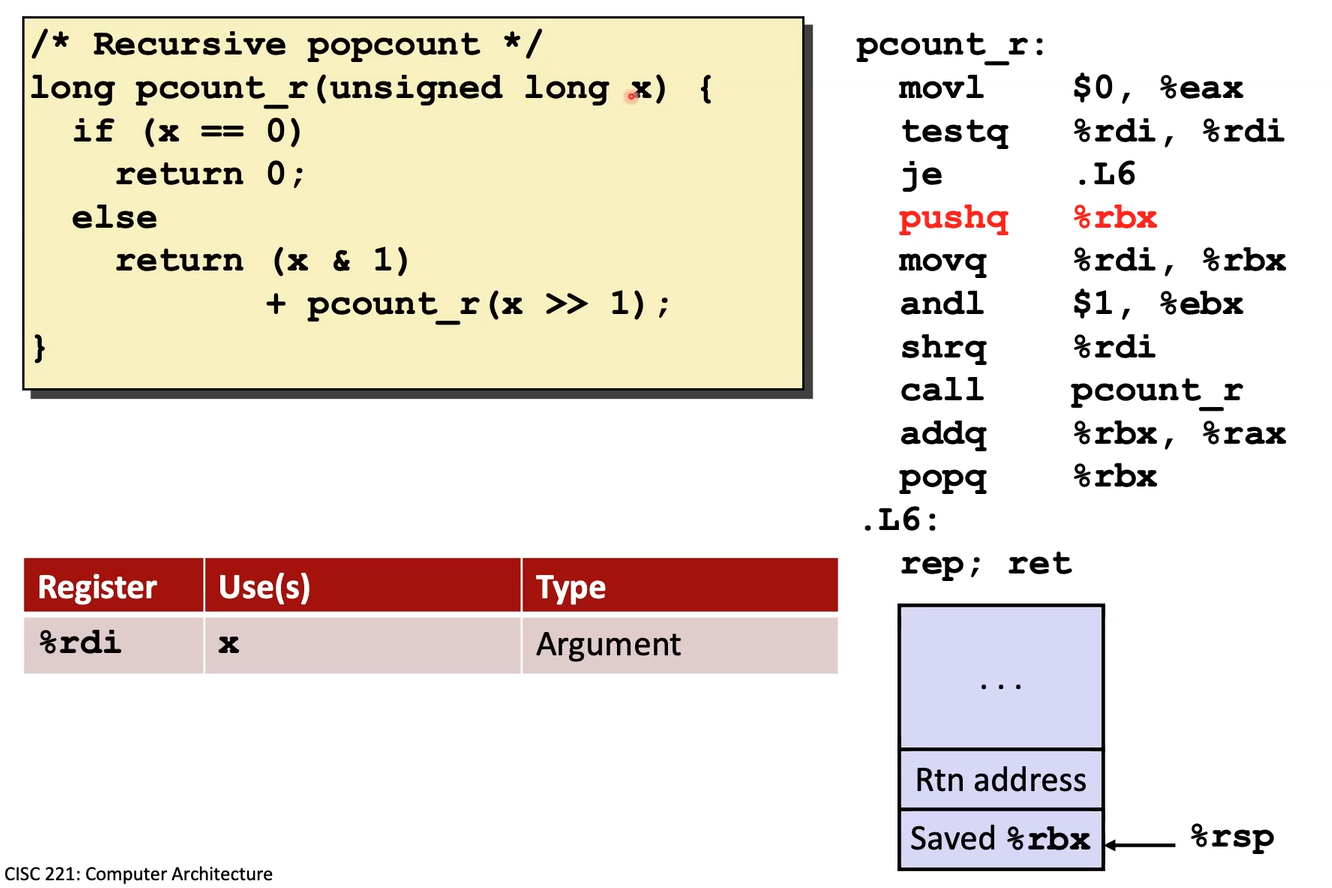
\includegraphics[scale = 0.2]{./figures/rec3}
        \caption{register save}
\end{figure}

\begin{figure}
        \centering
        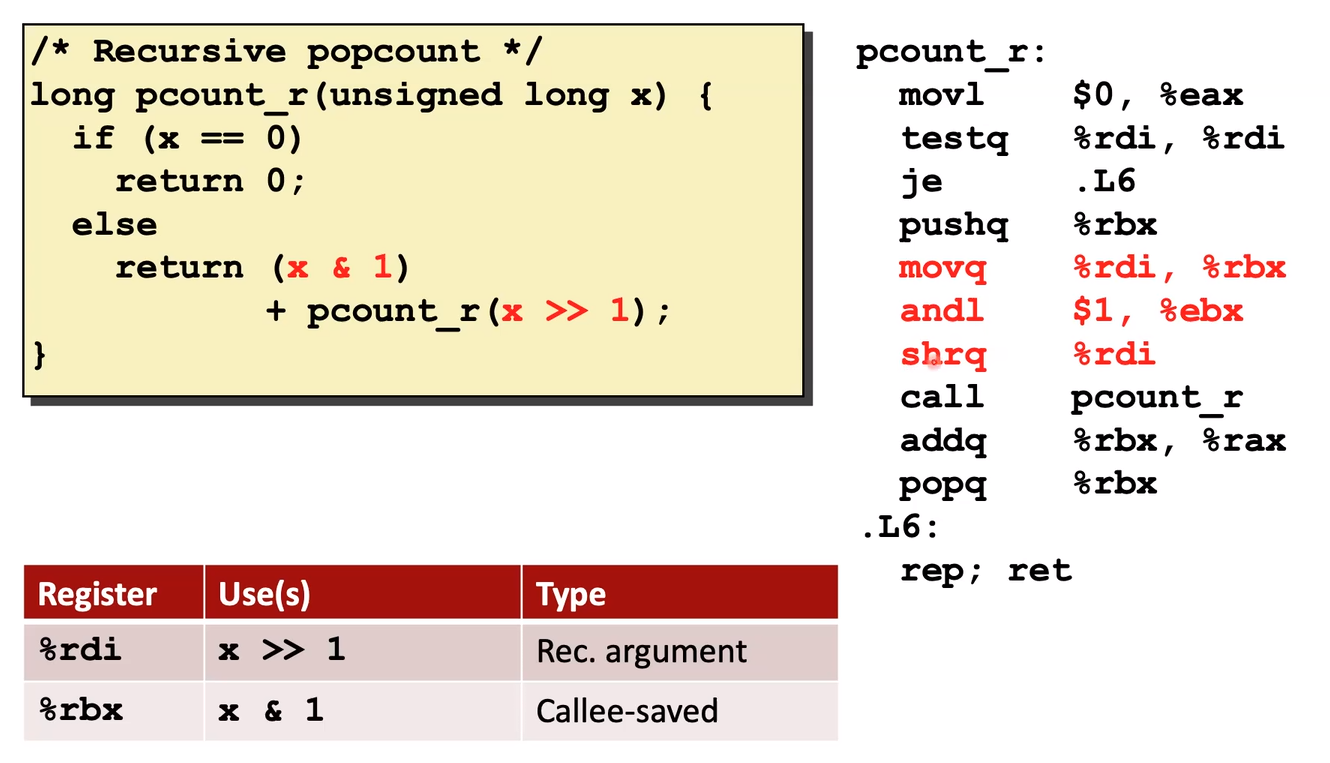
\includegraphics[scale = 0.2]{./figures/rec4}
        \caption{call setup}
\end{figure}

\begin{figure}
        \centering
        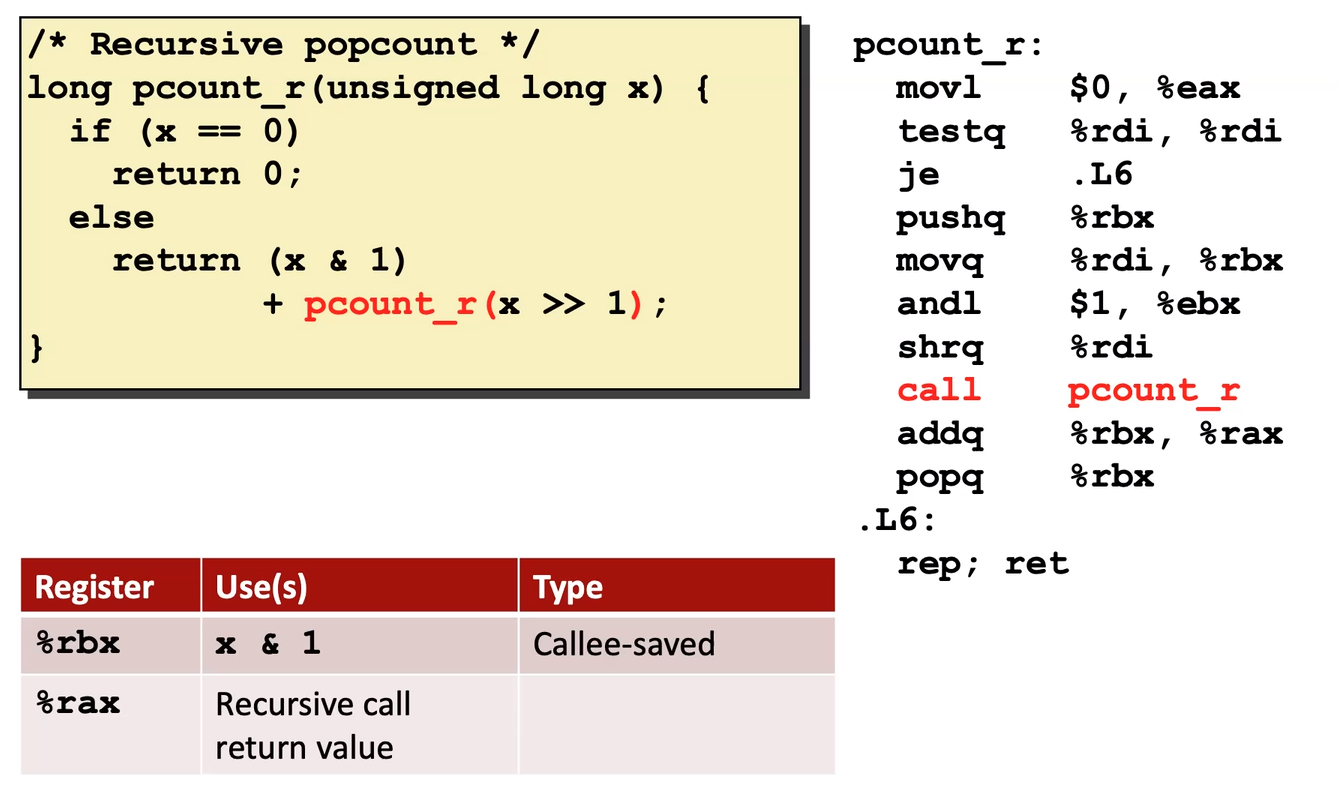
\includegraphics[scale = 0.2]{./figures/recOops}
        \caption{call}
\end{figure}

\begin{figure}
        \centering
        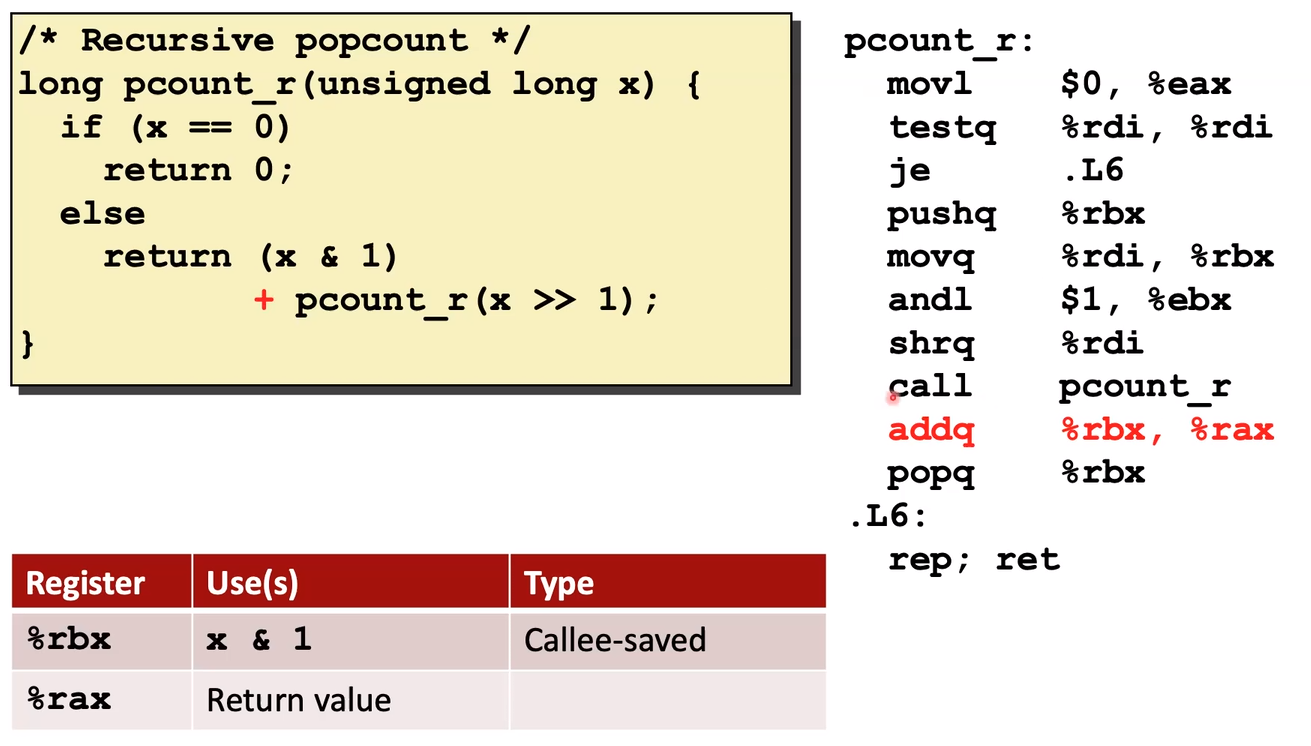
\includegraphics[scale = 0.2]{./figures/rec5}
        \caption{result}
\end{figure}

\begin{figure}
        \centering
        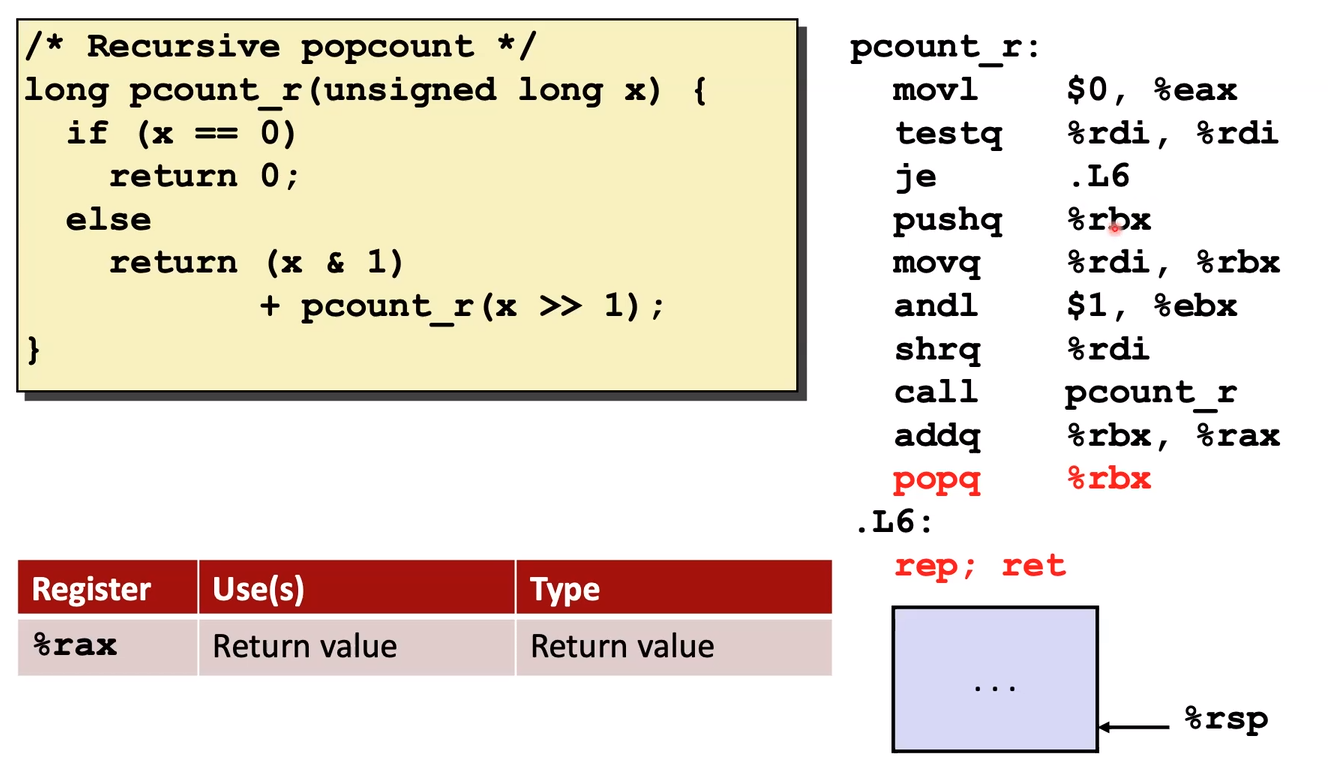
\includegraphics[scale = 0.2]{./figures/rec6}
        \caption{complete}
\end{figure}
\pagebreak

\subsection*{Observations about Recursion}
\begin{itemize}
        \item Handled without special consideration
        \begin{itemize}
                \item stack frames mean that each function call has private storage
                \begin{itemize}
                        \item saved registers and local variables
                        \item saved return pointer
                \end{itemize}
                \item register saving conventions prevent one function call from corrupting another's data
                \begin{itemize}
                        \item unless the C code explicitly does so (ie. programmer error)
                \end{itemize}
        \item stack discipline follows call / return pattern
                \begin{itemize}
                        \item if $P$ calls  $Q$, then  $Q$ returns before  $P$
                        \item Last In First Out
                \end{itemize}
        \item also works with mutual recursion (ie. $P$ calls  $Q$;  $Q$ calls  $P$)
        \end{itemize}
\end{itemize}

\section*{x86 Procedure Summary}
\begin{itemize}
        \item The stack is the right data structure for procedure call and return as it has all the safety
                needed to ensure consistent computations.
        \item recursion and mutual recursion are handled with normal calling conventions.
        \item \texttt{\%rax} always returns result
        \item pointers are addresses of values on the stack or globally.
\end{itemize}
\end{document}

